\chapter{Beleuchtung}  \label{beleuchten}
 
 In diesem Kapitel wird erklärt, wie unter Zuhilfenahme des radiometrischen und geometrischen Modells aus Kapitel \ref{kalibrierung} eine hochauflösende Beleuchtung mit einen Bildschirm erzeugt werden kann.
 Im weiteren Verlauf wird davon ausgegangen, dass die Position und Orientierung des Bildschirms im Raum zu jedem Zeitpunkt bekannt ist.
 Die Berechnung erfolgt mit Hilfe der Tracking-Stage, ARToolKit und dem geometrischen Modell aus Abschnitt  \ref{geometrisches_modell}.

 Damit mit dem Bildschirm an einer gegebenen Position eine einfallende Beleuchtung erzeugt werden kann, muss die Strahldichte berechnet werden, die von jedem Pixel in Richtung des Ursprungs emittiert werden soll.
 Diese gesamte, in die Szene einfallende Strahldichte wird dabei von einer Environment-Map vorgeben, anhand der sich, mit Hilfe des des geometrischen Modells, die \emph{benötigte} Strahldichte jedes einzelnen Bildschirmpixels berechnen lässt. 

 Daraufhin kann man das radiometrische Modell anwenden und für jeden Bildschirmpixel über das inverse Ansprechverhalten $v_{x,y}(l)$ den  benötigten Framebuffer-Werte berechnen, sodass die gewünschte einfallende Strahldichte erzeugt wird.
 Befindet sie sich innerhalb des vom Bildschirm darstellbaren Bereichs, so kann  man damit direkt eine Beleuchtung erzeugt.
 Der Dynamikbereich dieser Beleuchtung entspricht dabei genau dem des Bildschirms, weshalb sie hier als ``LDR-Beleuchtung'' bezeichnet wird.
 
 Das Kontrastverhältnis einer echten Umgebungsbeleuchtung ist jedoch weitaus größer als das eines gewöhnlichen Bildschirms. 
 In diesem Kapitel wird deshalb eine Methode vorgestellt, mit der sich der Dynamikbereich der erzeugten Beleuchtung durch eine zeitvariante Bildsequenz erhöhen lässt.
 Dieses Verfahren wird im Weiteren als ``HDR-Beleuchtung'' und die Sequenz als ``HDR-Sequenz'' bezeichnet.
 
 Damit eine Szene vollständig, also aus allen gewünschten Richtungen beleuchtet werden kann, müssen mit dem Bildschirm viele einzelne Teilbeleuchtungen erzeugt werden. 
 Dabei ist es wichtig, dass in jeder Teilbeleuchtung nur Licht emittiert wird, das noch nicht von einer anderen, vorangegangenen Teilbeleuchtung erzeugt wurde. 
 Es muss also zu jedem Zeitpunkt bekannt sein, welcher Teil der Beleuchtung schon hergestellt wurde und welcher noch nicht.

 Desweiteren soll die Beleuchtung von Hand durch einen Benutzer stattfinden, der den Bildschirm in einem dunklen Raum an die richtigen Stellen bewegt, und an jeder Position für mehrere Sekunden verharrt. 
 Der Bildschirm muss dabei möglichst präzise, mit einem festen Abstand und Winkel, zur Szene hin ausgerichtet werden.
 Aus diesem Grund wird ein in diesem Kapitel auch ein Beleuchtungsablauf vorgestellt, bei dem der Benutzer von einem Computerprogramm mit Audiosignalen geführt wird, die ihm eine falsche Bildschirmausrichtung signalisieren und ihn so bei der Beleuchtung unterstützen.
   Erst wenn sich der Bildschirm an eine akzpetablen Position befindet wird die Teilbeleuchtung hergestellt und aufgenommen.
  
%%%%%%%%%%%%%%%%%%%%%%%%%%%%%%%%%%%%%%%%%%%%%%%%
  
 \section {Benötigte Strahldichte} \label{projection}
  
   Sei $L_r$ nun die Matrix der \emph{benötigten Strahldichte}. 
   Sie gibt an, welche Strahldichte jedes Bildschirmpixel im Ursprung $O$ erzeugen soll.
   Der Abstand $r_l$ zwischen Ursprung und Bildschirm, sowie der Ausrichtungswinkel sind dabei, genau wie bei der radiometrischen Kalibrierung in Abschnitt \ref{radiometrisches_modell}, fix.
   
  Da die Positionen der Pixel im Raum bekannt sind, kann man $L_r$ prinzipiell anhand einer beliebigen Environment-Map berechnen:
     Die Weltkoordinaten der als Punktlichtquellen modellierten Pixel geben dabei die Richtung an, mit der das emittierte Licht in den Ursprung einfällt. 
    Mit dieser Lichtrichtung kann man dann die Strahldichte der Lichtquellen in der Environment-Map nachschlagen. 
 
   Sind die Punktlichtquellen regelmäßig auf einer Ebene angeordnet wie es bei einem Bildschirm der Fall ist, so ist es Sinnvoll eine Cube-Map als Environment-Map zu verwenden:
   Da Cube-Maps ebenfalls aus Ebenen bestehen, kann man $L_r$ mit perspektivischen Projektionen berechnen.
   Insbesondere ist es auch möglich, den Projektionsprozess umzukehren,  sodass man $L_r$ zurück auf eine Cube-Map projizieren kann.
    Damit lässt sich berechnen, welcher Teil der Environment-Map von einer Teilbeleuchtung hergestellt wurde.
 
    
      \begin{figure}[H]
    \centering
    \includegraphics[width=0.5\textwidth]{../graphics/beleuchtung/projektion_grey.png}
    \caption[Projektion von Cube-Map auf Bildschirmebene]{Die benötigte Strahldichte $L_r$ der Pixel wird mit Zentralprojektionen aus einer Cube-Map berechnet. Hierzu wird jede der sechs Seiten auf die Bildschirmebene projiziert, wobei der Augpunkt der Projektion im Ursprung $O$ liegt. 
    Die einzelnen Abbildungen ergeben aufsummiert die Strahldichteverteilung $L_r$.
    In der abgebildeten Bildschirmposition sind zwei Projektionen notwendig: Der Bereich $A$ von Seite $S_1$ wird auf $A'$, und $B$ von Seite $S_2$ wird auf $B'$ abgebildet. Das Ergebnis ist $L_r=A'+B'$.
    }
    \label{fig:projektion}
   \end{figure}
   
   Zur Berechnung von $L_r$ wird jede der sechs Cube-Map-Seiten einzeln auf den Bildschirm projiziert und das Ergebnis aufaddiert (Abbildung \ref{fig:projektion})  
   Der Augpunkt der Projektion befindet sich dabei im Ursprung $O$.
   Die perspektivische Projektion ist vollständig definiert, wenn für mindestens vier Punkte auf der Cube-Map-Ebene bekannt ist, auf welche Punkte der Bildschirmebene sie abgebildet werden.
   Wie in Abbildung \ref{fig:projektion_cubeside} dargestellt werden hierzu die vier Ecken der Bildschirmebene verwendet.
   Die jeweils korrespondierenden Punkte auf einer Seite der Cube-Map können durch einen Schnitt der Geraden, die durch die Ecken und den Ursprung verlaufen, berechnet werden.
   
   \begin{figure}[h]
    \centering
    \includegraphics[width=0.7\textwidth]{../graphics/beleuchtung/projektion_cubeside_grey.png}
    \caption[Projektion von Cube-Map-Seite auf Bildschirmebene]{Eine einzelne Seite $S_1$ der Cube-Map wird auf die Bildschirmebene projiziert:
     Die perspektivische Projektione ist dabei durch die vier Eckpunkte $e_1$ - $e_4$ des Bildschirms, und den vier Punkten $p_1$ - $p_4$ auf der Ebene $s_1$ festgelegt. 
    Die Punkte $p$ sind die Schnittpunkte der Geraden, die durch den Ursprung und die jeweilige Bildschirmecke $e$ verlaufen. 
    Sie liegen dabei zum Teil ($p_3$, $p_4$) auch außerhalb der eigentlichen Cube-Map-Textur (graue Ebene). In diesen Bereichen dürfen nur 0-Werte abgebildet werden (schraffierte Flächen).
    }
    \label{fig:projektion_cubeside}
   \end{figure}
    
    Mit diesem Schema kann man also $L_r$ anhand einer Environment-Map berechnen.
    Der Prozess lässt sich aber auch umkehren: Eine gegebene Bildschirmebene kann auf eine Cube-Map abgebildet werden.
    Hierzu wird einfach die Rolle der zwei Ebenen in der Projektion vertauscht und die Bildschirmebene einmal auf jede Cube-Map-Seite abgebildet.
    Damit ist es möglich, die von einem Bildschirm erzeugte Strahldichte in Form einer Environment-Map darzustellen und zu speichern.
    Dies wird für das korrekte Behandeln von Überlappungen beim Erzeugen einer vollständigen Beleuchtung in Abschnitt \ref{complete} benötigt.
  
  
%%%%%%%%%%%%%%%%%%%%%%%%%%%%%%%%%%%%%%%%%%%%555
  
 \section {LDR-Beleuchtung}  \label{ldr}
   Hat man die Strahldichteverteilung $L_r$ berechnet, so kann man sie mit einem radiometrisch kalibrierten Bildschirm erzeugen - vorrausgesetzt die Werte befindet sich innerhalb des darstellbaren Bereichs.
   Dieser Bereich wird durch die minimale Strahldichte $L_{0}$ und die maximale Strahldichte $L_{255}$ begrenzt, die die Pixel im Ursprung erzeugen können, wenn man den Framebuffer auf $V=0$ und $V=255$ setzt.
   Damit eine LDR-Beleuchtung erzeugt werden kann, muss also
   \begin{equation}
     L_0 \le L_r \le L_{255} 
   \end{equation}
   gelten, wobei mit " $\le$ " der elementweise Vergleich gemeint ist: Die Ungleichung muss für jedes Element in der Matrix erfüllt sein.
   Ist dies der Fall, so kann man den Framebuffer $V$ berechnen, indem man das inverse Ansprechverhalten auf jedes Pixel einzeln anwendet:
   \begin{equation}
     \forall (x,y): \ \ \  V(x,y) = v_{x,y}(L_r(x,y))
   \end{equation}

%berechnung von v
   In Abschnitt \ref{display_response} wurde das inverse Ansprechverhalten $v_{x,y}$ nicht pro Pixel, sondern pro Patch berechnet und liegt somit nur in einer niedrigen räumlichen Auflösung vor.
   Die Ansprechkurven jedes Pixels werden deshalb mit Hilfe einer Interpolation berechnet. 
   Das kann zur Laufzeit geschehen, sodass nicht alle Kurven im Speicher gehalten werden müssen. 

   Zur Erklärung des Interpolation wird nun Abbildung \ref{fig:interpolation} betrachtet.
   Sei $v_{ (p_{i,j}) } (l)$ das inverse Ansprechverhalten eines Patches $p_{i,j}$, und $(x_{i,j},y_{i,j})$ sein Mittelpunkt in Pixelkoordinaten.
   Für die Interpolation wird angenommen, dass $v_{x_{i,j},y_{i,j}}(l) = v_{ (p_{i,j}) }(l) $ gilt.
   Dem mittleren Patchpixel wird also genau das Ansprechverhalten zugeschrieben, das durch Mittelung der benachbarten Pixel berechnet wurde. 

   Die Ansprechkurve eines Pixels an der Position $(x,y)$ kann dann durch eine bilineare Interpolation aus den vier Kurven der benachbarten Patches berechnet werden.
   Die vier Patchnachbarn eines Pixels sind die Patches, dessen Mittelpunkt am nächsten an $(x,y)$ liegt.
 
   Seien $p_{n,m}$,\hspace{2mm}  $ p_{n+1,m}$,\hspace{2mm} $ p_{n,m-1}$,\hspace{2mm} $ p_{n+1,m-1}$ nun die vier Patchnachbarn des Pixels $(x,y)$.
   Die Kurve $v_{x,y}(l)$ des Pixels berechnet sich dann durch eine bilineare Interpolation von  $v_{p_{n,m}}(l)$,\hspace{2mm} $v_{p_{n+1,m}}(l)$,\hspace{2mm}   $  v_{p_{n,m-1}}(l)$,\hspace{2mm} $ v_{p_{n+1,m-1}}(l)$.
   Die Gewichtungen in der Interpolation sind dabei durch den Abstand des Pixels zu den vier Patchmittelpunkten gegeben.

  \begin{figure}[h]
    \centering
    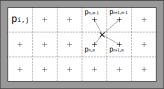
\includegraphics[width=0.5\textwidth]{../graphics/beleuchtung/interpolation.svg}
    \caption[Interpolation des Per-Pixel-Ansprechverhaltens]{ Bilineare Interpolation des Per-Pixel-Ansprechverhaltens aus dem Per-Patch-Ansprechverhalten:
          %Bei der Kalibrierung wurde für jeden Patch $p_{i,j}$ ein eigenes Ansprechverhalten berechnet.
          Es wird angenommen, dass das Ansprechverhalten eines Patches $p_{i,j}$ für den jeweiligen Mittelpunkt (\textbf{+}) gültig ist.
          Die Ansprechkurve eines beliebigen Pixels ($\times$) kann dann anhand einer bilinearen Interpolation aus den Kurven der benachbarten Patches berechnet werden.
          }
    \label{fig:interpolation}
   \end{figure}



%   Wie groß die Patchgröße $k$ gewählt werden darf hängt von der Charakteristik des Bildschirms ab.
%   Wird $k$ zu groß gewählt, so kann es passieren dass die Annahme der Stetigkeit durch die Bilinearen Interpolation verletzt wird; wird es zu klein gewählt, so erhöht sich das Rauschen in den Messergebnissen bei der Kalibrierung.
%    
%   In der Praxis haben sich Patches mit einer Größe von $5-10 mm$ bewährt. 
%   Bei gängiger Pixeldichte (96-120 dpi) entspricht dies einem Bereich von 20-50 Pixel.  
 
%dynamikbereich D
    Der Dynamikbereich einer LDR-Beleuchtung orientiert sich an der minimalen und der maximalen Strahldichte die mit dem Bildschirm herstellbar ist. 
    Hier ist es wichtig, dass nur die Strahldichte betrachtet wird, die von \emph{jedem} Pixel erzeugt werden kann.
    Der Dynamikbereich $R$, den man mit einer LDR-Beleuchtung erreichen kann, lautet also
     \begin{equation}
       R=\frac{\min{(L_{255})}}{\max{(L_{0})}}
     \end{equation}
    wobei $\min()$ und $\max()$ das kleinste und das größte Element der Matrizen bezeichnet.
    
 
    Im nächsten Abschnitt wird gezeigt, dass es durch Aufnahme eines Darkframes möglich ist, $L_{0} = 0$ zu erreichen.
    Dies ist eine Vorraussetzung für die HDR-Beleuchtung im darauf folgenden Abschnitt.  

%%%%%%%%%%%%%%%%%%%%%%%%%%%%%%%%%%%%%%%%%%%%%%%%%%%%%%%%%%%%%%%
   
\subsection{Reduktion von $L_{0}$}   \label{reduktion} 
     Die minimale Strahldichte $L_{0}$, die ein Bildschirm erzeugen kann, entspricht seinem Schwarzwert und begrenzt den Dynamikbereich maßgeblich.
     Da das Licht des Bildschirm jedoch nicht von einem Menschen, sondern von einer Kamera wahrgenommen werden soll, kann $L_{0}$ bei fixer Bildschirmposition durch ein zweites Foto vermessen, und von der eigentlichen Aufnahme abgezogen werden.
     Das Prinzip ist analog zu der in Kapitel \ref{display_response} vorgestellten Darkframe-Aufnahme, jedoch dass in diesem Fall die Hintergrundbeleuchtung angeschaltet bleibt und der Framebuffer auf $V=0$ gesetzt wird.

     Im Rest der Arbeit wird davon ausgegangen, dass zu jeder fotografierten Teilbeleuchtung $T$ auch ein Darkframe $D$ aufgenommen wird. 
     Subtrahiert man das Darkframe von der eigentlichen Aufnahme $T$, so erhält man das Bild $T'$:
    \begin{equation}
        T'  = T - D
    \end{equation}

    Mit der Darkframesubtraktion ändert sich die effektiv herstellbare, minimale und maximale Strahldichte des Bildschirms: 
    \begin{eqnarray*}
        L'_{0} &=& L_0 - L_0 = 0 \\
        L'_{255} &=& L_{255} - L_0
    \end{eqnarray*}
    
     Der Wertebereich des Ansprechverhaltens $l_{x,y}(v)$ eines Pixels $(x,y)$ verschiebt sich ebenfalls um $l^0_{x,y} = L_0(x,y)$.
     Das inverse Ansprechverhalten lautet also 
     \begin{equation}
        v'_{x,y}(l) = v_{x,y}(l+l^0_{x,y}) \\
    \end{equation}
     und kann zur Laufzeit aus $v_{x,y}(l)$ berechnet werden.
    
%dynamikbereich

     Der Dynamikbereich des Bildschirms verändert sich bei einer Darkframesubtraktion ebenfalls, da zum Einen der kleinste darstellbare Wert nicht mehr vom Schwarzwert $V=0$, sondern von $V=1$ bestimmt wird (siehe Definition des Dynamikbereichs in Abschnitt \ref{dynamikbereich}),
     und zum Anderen auch die maximale Strahldichte verringert wird.
     Sei $L_{1}$ nun die Strahldichte, die bei einem Framebuffer $V=1$ vom Bildschirm im Ursprung erzeugt wird.
     Die kleinste erzeugbare Strahldichte $L'_{1} > 0$ ist dann durch
     \begin{equation}
        L'_{1} = L_{1} - L_0\\
    \end{equation}
    gegeben.
     Der Dynamikbereich eines Bildschirms, im Falle einer Darkframesubtraktion, lautet also 
     \begin{equation}
       R'=\frac{\min{(L_{255}-L_{0})}}{\max{(L_{1}-L'_{0})}} = \frac{\min{(L'_{255})}}{\max{(L'_{1})}}
     \end{equation}

     Ob $R'>R$ oder $R'<R$ gilt hängt von dem Verhältnis zwischen $L_{1}$ und $L_{0}$ ab. 
     Bei LCD-Bildschirmen ist der der Schwarzwert $L_{0}$ meist deutlich größer als $L'_{1}$, sodass $R' > R$ ist. 
     
     Es sei anzumerken dass diese Betrachtungsweise nur dann korrekt ist, wenn das Sensorrauschen der Kamera vernachlässigbar klein ist.
     Dies ist in der Praxis mit einem großen Aufwand verbunden, da es sich bei $L_{0}$ und insbesondere bei $L'_{1}$ um sehr kleine Lichtmengen handelt.
     Im weiteren Verlauf wird deshalb davon ausgegangen, dass alle Aufnahmen rauschfrei sind. 
     

%%%%%%%%%%%%%%%%%%%%%%%%%%%%%%%%%%%%%%%%%%%%%%%%%%%%%%%%%%%%%%%

 \section {HDR-Beleuchtung} \label{hdr}

    Der Dynamikbereich einer LDR-Beleuchtung ist stark eingeschränkt, besonders wenn ein Bildschirm mit starker Blickwinkelabhängigkeit verwendet wird.
    Es ist jedoch möglich das Kontrastverhältnis mit einer zeitvarianten Sequenz zu vergrößern:
    Während einer Langzeitbelichtung von mehreren Sekunden lassen sich nämlich nicht nur ein einzelnes, sondern gleich viele unterschiedliche Bilder nacheinander anzeigen.
    Bildlich gesprochen kann man so  die Strahldichte $L_r$ ``über die Zeit verteilen''. 
    Es ist also eine feinere Regelung der emittierten Strahldichte möglich - insbesondere lassen sich so Werte kleiner als  $L'_{1}$ herstellen.
    
    Im Folgenden wird gezeigt, wie man so eine zeitvariante Sequenz konstruieren kann und wie sich damit der Dynamikbereich der erzeugten Beleuchtung vergrößern lässt.
    Sie wird hier als ``HDR-Sequenz'' bezeichnet, ein einzelnes Bild innerhalb der Sequenz  als ``Frame''.
   
% annahme: belichtungszeit konstant, anzahl frames variabel, frames gleichverteilt ueber zeit
    Angenommen wir haben einen Bildschirm und setzten den Framebuffer auf $V=1$. 
    Unter Einsatz der Darkframesubtraktion aus Abschnitt \ref{reduktion} messen wir, bei einer Belichtungszeit von $t$ Sekunden, die Strahldichteverteilung $L'_{1}$ im Ursprung.
    Zeigt man in der Zeit $t$ statt einem statischen Bild eine zeitvariante Sequenz aus $m$ Frames an, die dabei gleichmäßig über die Zeit verteilt sind, so ist die kleinste Strahldichte, die in \emph{einem Frame} hergestellt werden kann, $L'_{1}/m$, und die größte ist $L'_{255}/m$.
    Dies ist möglich, da mit der Darkframesubtraktion aus Kapitel \ref{reduktion},  in einem Frame auch \emph{gar kein} Licht emittiert werden kann ($L'_{0} = 0$).
    
    Würde man also $L'_{1}/m$ mit einer HDR-Sequenz der Größe $m$ erzeugen, so wäre genau in einem der Frames $V=1$, und in allen anderen $V=0$. 
    Bei  $L'_{255}$ hingegen wäre in allen Frames $V=255$, die maximale erzeugbare Strahldichte ändert sich also nicht.
 
    Der Dynamikbereich, der mit einer HDR-Sequenz der Länge $m$ erreicht werden kann, lautet also
    \begin{equation}
      R_{HDR} = \frac{ \min{ (L'_{255}}) } { \max{ (L'_{1})}/m} = mR'
    \end{equation}
    und ist damit genau $m$ mal größer als $R'$.
 
    Im Folgenden wird ein Algorithmus vorgestellt, mit dem eine HDR-Sequenz berechnet werden kann.
    Dazu wird die Belichtungszeit $t$ als gegeben betrachtet. 
    Sie wird vom Benutzer festgelegt, und orientiert sich an der Zeit die für eine einzelne Teilbeleuchtung zur Verfügung steht.
    Für die Anzeige der HDR-Sequenz kann die höchstmögliche Framerate $1/t_{max}$ gewählt werden, die mit dem Anzeigegerät ruckelfrei darstellbar ist. Es wichtig, dass jedes Frame genau $t/m$ Sekunden auf dem Bildschirm verweilt, da sonst entweder zu viel oder zu wenig Licht emittiert wird.

    Die Länge der HDR-Sequenz, die sich in der Zeit $t$ erzeugen lässt, ist also durch 
    \begin{equation}
     m=t/t_{max}
    \end{equation}
    gegeben und somit auch festgelegt.

    Die Aufgabe des Algorithmus ist es, eine gegebene Strahldichte $L_r$ auf eine HDR-Sequenz der Länge $m$ zu verteilen. 
    Die Grundidee des Verfahrens soll anhand eines einfachen, eindimensionalen Beispiels verdeutlicht werden.
    In den Graphen in Abbildung \ref{fig:hdr_graph_example}) ist die Strahldichte von sechs fiktiven Pixeln dargestellt.
    Auf der linken Seite befindet sich die zu erzeugende Strahldichte $L$, die vom HDR-Algorithmus auf die drei Frames auf der rechten Seite verteilt wird. 

   \begin{figure}[h]
    \centering
    
\includegraphics[width=\textwidth]{../graphics/beleuchtung/hdr_sequence_example.svg}
    \caption[1D-Beispiel einer HDR-Sequenz]{Der HDR-Algorithmus verteilt die Strahldichte $L$, hier für sechs Pixel dargestellt, auf drei Frames. Jedes Frame wird genau $t/3$ Sekunden lang angezeigt, sodass in einer Langzeitbelichtung von $t$ Sekunden in der Summe genau $L$ erzeugt wird.
     }
    \label{fig:hdr_graph_example}
   \end{figure}
  
   Damit $L_r$ auch innerhalb der gegebenen Zeit $t$ erzeugt werden kann, muss sie skaliert werden.
   Hierzu wird ein Faktor $f$ so gewählt dass 
    \begin{equation}
      \frac{L_{r}}{f} \le L'_{255}
    \end{equation}
    gilt.
    Der Dynamikbereich von $L_{r}$ wird quasi in den der HDR-Sequenz eingepasst, sodass eine Beleuchtung mit dem höchstmöglichen Kontrast erzeugt werden kann, die mit dem Bildschirm in  $m$ Frames möglich ist.
    Den Faktor $f$ berechnet man, indem das größte Element der elementweisen dividierten Matrizen $L_{r}/L'_{max}$ sucht:
    \begin{equation}
      f=\max{(\frac{L_{r}}{L'_{255}})}
    \end{equation}


    Der HDR-Algorithmus basiert auf einem einfachen iterativen Verfahren, bei dem $L_r/{f}$ schrittweise auf die Frames verteilt wird.
    Dazu wird eine temporäre Matrix $L_t=L_{r}/f$ initialisiert, und in einer Schleife $m$-mal $L_t=L_t-L'_{255}/m$ berechnet. 
    In jedem Schritt lässt sich dann ein Frame aufbauen, indem man über alle Pixel $(x,y)$ iteriert und die ``restliche'', noch nicht emittierte Strahldichte  $L_t(x,y)$ betrachtet.

    Dabei müssen drei unterschiedliche Fälle behandelt werden:
    \begin{itemize}
       \item{ Falls  $L_t(x,y) \geq L'_{255}/m$ ist, so muss  $V(x,y)=255$  sein.}
       \item{ Falls  $L_t(x,y) \leq 0$ ist, so muss  $V(x,y)=0$  sein.}
       \item{ In allen anderen Fällen ist $L_t(x,y)$ vom Bildschirm darstellbar:  $V(x,y)=v'_{x,y}(L_t(x,y))$}
    \end{itemize}
  
  
    Betrachtet man den Wert $V(x,y)$ eines Pixels über alle Frames einer so erzeugten HDR-Sequenz, so ist er zuerst über mehrere Frames $V(x,y)=255$, dann wird in genau einem Frame einmal das inverse Ansprechverhalten $v'{x,y}$ angewendet, und in den restlichen  Frames ist $V(x,y)=0$.
    Der Algorithmus lässt sich also optimieren indem man die zwei Schleifen vertauscht, und in der äußeren über die Pixel statt über die Frames iteriert.
    Das hat den Vorteil, dass abgebrochen werden kann sobald ein Pixel die zu erzeugende Strahldichte erreicht hat.
    
    Der HDR-Algorithmus kann also wie im folgenden Pseudocode dargestellt implementiert werden:

   \vspace{3mm}

    \begin{algorithmic} 
      \State $ \forall n<m: F_n \gets 0$                        \Comment {Alle Frames auf Null setzen}
      \State $ L \gets \frac{1}{f}L_{r}$                        \Comment {Strahldichte skalieren}
         \For { $(x,y) = (0,0)$ to $(w-1,h-1)$ } 	        \Comment{ für alle Pixel ..}
            \For { $n=0$ to $(m-1)$ }     	                \Comment{ für alle Frames ..} 
                \If {$L(x,y) \geq \frac{1}{m}L'_{255}(x,y)  $}  \Comment { maximale Strahldichte emittieren}
                  \State { $F_n(x,y) \gets 255$ }  
                  \State { $L(x,y) \gets L(x,y) - \frac{1}{m}L'_{255}(x,y)$ }  
                \ElsIf { $L(x,y) < \frac{1}{m}L'_{255}(x,y)$ } \Comment { Ansprechverhalten anwenden }
                  \State { $F_n(x,y) \gets v'_{x,y}(L(x,y))$ }
                  \State { $L(x,y) \gets 0 $ }
                \Else                                            \Comment { kein Licht emittieren } 
                  \State { $F_n(x,y) \gets 0$ }  
                  \State { \textbf{break} }                               \Comment { Abbruch, sobald $L(x,y)=0$}
                \EndIf
             \EndFor  
          \EndFor
    \end{algorithmic} 

   Die Ausgabe des HDR-Algorithmus, die für den Laptopbildschirm berechnet wurde, ist in den Abbildungen \ref{fig:hdr_frames_example_uniform} und \ref{fig:hdr_frames_example} zu sehen. 
   In \ref{fig:hdr_frames_example_uniform} kann man sehen, dass mit einer HDR-Sequenz automatisch die ungleichmäßige Hintegrundbeleuchtung des Bildschirms ausgeglichen wird.
   Abbildung \ref{fig:hdr_frames_example} zeigt hingegen eine HDR-Sequenz der Länge 50, wobei $L_r$ von einer echten HDR-Umgebungsbeleuchtung vorgegeben wurde. 
   Der dargestellte Ausschnitt besitzt dabei einen Dynamikbereich von 10000:1.
   
  
   \begin{figure}[h]
    \centering
       \includegraphics[width=0.3\textwidth]{../graphics/hdr_beleuchtung/white_frame_0.png} 
       \includegraphics[width=0.3\textwidth]{../graphics/hdr_beleuchtung/white_frame_1.png} 
       \includegraphics[width=0.3\textwidth]{../graphics/hdr_beleuchtung/white_frame_2.png} 
    \caption[HDR-Frames: Uniforme Strahldichte]{ Ausgabe vom HDR-Algorithmus: Eine uniforme Strahldichte ($L_r=1$) wird auf drei Frames verteilt. Man kann gut erkennen, dass in den Randbereichen mehr Licht erzeugt wird als in der Mitte, da der Bildschirm dort eine niedrigere maximale Strahldichte $L_{255}$ besitzt (siehe Abbildung \ref{fig:lenovo_responses}).
    } 
    \label{fig:hdr_frames_example_uniform}
   \end{figure}

  
   \begin{figure}[h]
    \centering
    \includegraphics[width=0.3\textwidth]{../graphics/hdr_beleuchtung/ennis_frame_0_small.png}
    \includegraphics[width=0.3\textwidth]{../graphics/hdr_beleuchtung/ennis_frame_1_small.png}
    \includegraphics[width=0.3\textwidth]{../graphics/hdr_beleuchtung/ennis_frame_2_small.png}
    \includegraphics[width=0.3\textwidth]{../graphics/hdr_beleuchtung/ennis_frame_29_small.png}
    \includegraphics[width=0.3\textwidth]{../graphics/hdr_beleuchtung/ennis_frame_39_small.png}
    \includegraphics[width=0.3\textwidth]{../graphics/hdr_beleuchtung/ennis_frame_49_small.png}
    \caption[HDR-Frames: Echte Szene]{Ausgabe vom HDR-Algorithmus: Dargestellt sind die Pixelwerte ($V$) von sechs Frames (1, 2, 3, 30, 40 und 50) einer HDR-Sequenz der Länge 50. 
    Bei der Environment-Map handelt es sich um das ``Ennis-Brown House'' aus der Debevec HDR Light Probe Gallery \cite{lightprobe_gallery}. 
    Der Ausschnitt zeigt ein Raum, durch dessen Fenster die Sonne hineinscheint. Der Wertebereich umfasst dabei 5 Größenordnungen.
    Es ist gut zu sehen dass die Pixel, die eine größere Strahldichte erzeugen sollen, über einen längeren Zeitraum Licht emittieren. 
    Kleine Strahldichtewerte werden dagegen mit den ersten Frames der Sequenz hergestellt. 
    Es kommt dabei zu einer Auftrennung der Farben, da die Farbkanäle unabhängig behandelt werden.
    }
    \label{fig:hdr_frames_example}
   \end{figure}
   
   

   Der Algorithmus wurde für diese Arbeit mit OpenCV auf der CPU implementiert. 
   Er kann aber auch problemlos auf einer GPU, beispielsweise als Pixel-Shader, implementiert werden.
   Eine CPU-basierte Implementierung ist für den Beleuchtungsablauf, der im nächsten Abschnitt \ref{illuminate} vorgestellt wird, jedoch vollkommen ausreichend, da ausreichen Rechenzeit zur Verfügung steht 
  

%%%%%%%%%%%%%%%%%%%%%%%%%%%%%%%%%%%%%%%%%%%%%%%%%%%%%%%%%%%%%%%

 \section{Vollständige Beleuchtung} \label{complete}
   
   Ist die Bildschirmposition im Raum bekannt, so kann mit den in Abschnitt \ref{projection} - \ref{hdr} vorgestellten Methoden eine einzelne Teilbeleuchtung erzeugt werden. 
   Wenn sich der Bildschirm dabei auf der vorgesehenen Halbkugel befindet, so kann seine Position zu jedem Zeitpunkt anhand der  Tracking-Stage aus Kapitel \ref{position} berechnet werden.
   Die Szene kann somit durch einen Benutzer aus jeder Richtung beleuchtet werden.
  
   Bevor mit diesem System jedoch eine vollständige, zusammenhängende Beleuchtung erzeugt hergestellt kann sind noch mehrere Hindernisse zu bewältigen:  
   Zum Einen darf in jeder Teilbeleuchtung nur das Licht emittiert werden, das noch nicht von einer vorangegangenen Bildschirmposition erzeugt wurde. 
   Es muss also protokolliert werden, welche Teile der Beleuchtung schon hergestellt wurden und welche noch nicht. 
   Ansonsten kann es passieren, dass ein Teil mehrfach erzeugt und somit zu viel Licht emittiert wird - die Teilbeleuchtungen \emph{überlappen} sich.

   Zum Anderen muss der Benutzer den Bildschirm immer mit dem Abstand und dem Winkel zur Szene hin ausrichten, die bei der radiometrischen Kalibrierung festgelegt wurden.
    Da der Beleuchtungsprozess ``blind'' in einem abgedunkelten Raum stattfindet, wird der Benutzer durch ein Programm geführt.
      
   Im nächsten Abschnitt wird nun zuerst das Behandeln von Überlappungen erklärt, und danach auf den Beleuchtungsablauf eingegangen.
  
%%%%%%%%%%%%%%%%%%%%%%%%%%%%%%%%%%%%%%
  \subsection{Behandeln von Überlappungen} \label{overlap}
   
   In jeder Teilbeleuchtung  darf immer nur der Teil der Beleuchtung hergestellt werden, der noch nicht in einer Vorangegangenen Bildschirmposition erzeugt wurde.
   Da die Tracking-Stage und die Positionsberechnung gewissen Toleranzen unterliegt, kann die Bildschirmposition in der Praxis nie exakt berechnet werden und weicht immer von der tatsächlichen Position ab.
   Man kann also nie genau wissen, welcher Teil der Beleuchtung tatsächlich erzeugt werden muss beziehungsweise erzeugt wurde.
   Desweiteren ist der Bildschirm nicht fix - der Benutzer wackelt und driftet während der Beleuchtung langsam von der initialen Position ab. 
   In der Praxis kommt es also, selbst wenn Buch über die Beleuchtung geführt wird, zu Überlappungen bei Teilbeleuchtungen.
   
   Überlappungen äußern sich dadurch, dass an einer Stelle zu viel Licht und an einer anderen Stelle zu wenig Licht abgegeben wird.   
   Wenn sich zwei Beleuchtungen überlappen, so wird im schlimmsten Fall an einer Stelle die doppelte Strahldichte erzeugt, und an einer anderen gar keine. 
   Auf spiegelnden Oberflächen und im Backdrop werden sie deshalb als helle und dunkle Artefakte sichtbar.

   Ein sehr ähnliches Problem tritt bei der Kalibrierung von Multi-Projektor-Systemen auf: Dort sollen mehrere Projektoren so angeordnet und kalibriert werden, dass sie gemeinsam ein zusammenhängendes Bild erzeugen.
   Es wird üblicherweise durch einen weichen Übergang (engl: ``feathering'') zwischen den Projektobildern gelöst \cite{Raskar_1999}.
   Die Pixel, die sich überlappen werden hierzu mit einer linearen Rampe oder einer Cosinusfunktion multipliziert, die so gewählt ist, dass bei der Überlappung in der Summe der geforderte Helligkeitswert erzeugt wird.
   In der Praxis ist es meist ausreichend, wenn linear zwischen den Projektorbildern übergegangen wird  \cite{Raskar_1999}.

   In dieser Arbeit werden einfache lineare Rampe verwendet.
   Da es bei einer vollständigen Beleuchtung an jeder Kante der Anzeigefläche zu einer Überlappung kommt, werden alle vier Ränder mit linearen ausgeblendet.
   Die Breite der Rampen  sollte dabei deutlich größer sein als die Abweichung, die bei der Positionsberechnung auftreten.
   
   Sie werden werden in einer Alphamaske $M$  gespeichert und bei Beginn der Beleuchtung vorberechnet.
   Bei der Strahldichteberechnung wird  $L_r$ dann elementweise mit $M$ multipliziert, und die Matrix 
   \begin{equation}
      L'_r = L_r \cdot M
   \end{equation} 
   berechnet, die als die Eingabe für den HDR-Algorithmus dient.

   Dieser Vorgang ist in Abbildung \ref{fig:overlap_flow} als Flussdiagramm dargestellt.
   Dabei bezeichnet $E$ die Environment-Map, welche die Beleuchtung vorgibt, und $P$ steht für die Zentralprojektionen aus Kapitel \ref{projection}. 
   Die untere Hälfte des Diagramms zeigt wie berechnet wird, welcher Teil der Umgebungsbeleuchtung erzeugt wurde:
   Die Maske $M$ wird zuerst invertiert und dann mit der inversen Projektion $P^{-1}$ (siehe Abschnitt \ref{ldr}) von der Bildschirmebene auf eine Cube-Map $E_M$ abgebildet.
   $E_M$ gibt an, welcher Anteil der Environment-Map in einer Teilbeleuchtung erzeugt wurde.
   Die Beleuchtung, die noch erzeugt werden muss, ergibt sich dann durch eine elementweise Multiplikation von $E$ und $E_M$.
   Sie dient als Eingabe für die nächste Teilbeleuchtung.
      
   \begin{figure}[h]
    \centering
    \includegraphics[width=0.8\textwidth]{../graphics/beleuchtung/overlap_flow.png}
    \caption[Flussdiagramm: Überlappungsbehandlung]{ Die Überlappungsbehandlung als Flussdiagramm:
       Ausgehend von einer Cube-Map $E$ wird mittels perspektivischen Projektionen (hier mit $P$ bezeichnet) die Strahldichteverteilung $L_r$ berechnet. 
       Multipliziert mit der Maske $M$ ergibt sich die Matrix $L'_r$, die  als Eingabe für den HDR-Algorithmus dient.
       Die invertierten Maske $(1-M)$ wird mit einer inversen Projektion $P^{-1}$ auf eine Cube-Map $E_M$ abgebildet.
       Sie gibt an, welche Teile von $E$ in den folgenden Teilbeleuchtungen erzeugt werden müssen. Mit $E = E \cdot E_M$ ist also die Beleuchtung für den nächsten Durchlauf gegeben.
     }
    \label{fig:overlap_flow}
   \end{figure}


%%%%%%%%%%%%%%%%%%%%%%%%%%%%%%%%%%%%%%%%%%%%%%%%%%%%%%%%%%%%%%%

 
  \subsection{Ablauf}   \label{illuminate}
    
   Im Folgenden wird der Ablauf des Beleuchtungsprozesses erläutert. 
   Er ist dabei in Form eines einzigen Programmes implementiert, das auf dem Laptop läuft.
   Es steuert alle Hardwarekomponenten des System (Bildschirm, Webcam, DSLR-Kamera) und berechnet, erzeugt und fotografiert die Teilbeleuchtungen.
   Es sorgt nebenbei auch dafür, dass die Annahmen die in der radiometrischen Kalibrierung getroffen wurden, zu jedem Zeitpunkt mit einer gewissen Toleranz eingehalten werden.
  
   Abbildung \ref{fig:ablauf} zeigt den Ablauf einer vollständigen Beleuchtung als Flussdiagramm.
   Jede Teilbeleuchtung wird dabei auf die gleiche Art und Weise durchgeführt: 
   Als erstes bewegt der Benutzer den Bildschirm an eine Position und hält ihn ruhig.
   Die Position muss dabei die Annahmen erfüllen, die bei der radiometrischen Kalibrierung getroffen wurden.
   Der Abstand zwischen Szenenursprung und Bildschirmmittelpunkt muss $r_l$ betragen, und die Ebene muss mit dem richtigen Winkel ausgerichtet sein. 
   Ist dies nicht der Fall, so wird ein Audiosignal ausgegeben das den Benutzer anweist, wie er eine akzeptable Position erreichen kann (``näher kommen'', ``weiter entfernen'' und  ``Winkel einstellen'').
   Sobald die Position sich innerhalb einer gewissen Toleranz befindet, beginnt die Aufnahme einer Teilbeleuchtung.
   Die DSLR wird dabei direkt vom Programm über USB gesteuert, wozu ein separater Thread eingesetzt wird.
  
  \begin{figure}[H]
    \centering
    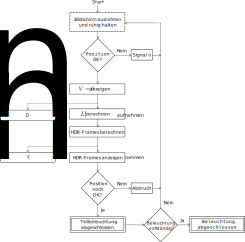
\includegraphics[width=0.8\textwidth]{../graphics/beleuchtung/ablauf.svg}
    \caption[Flussdiagramm: Beleuchtungsablauf]{Beleuchtungsablauf als Flussdiagramm: In jedem Durchlauf wird eine Teilbeleuchtung erzeugt. Dazu bewegt der Benutzer den Bildschirm an eine Position und hält ihn dort ruhig. Weicht die Position zu stark von der Vorgabe (Abstand, Winkel) ab, so wird ihm signalisiert wie er die richtige Position finden kann. Sobald er sie erreicht hat, wird der Bildschirm auf Schwarz geschaltet und  $L'_r$ sowie die HDR-Frames berechnet. 
    Gleichzeitig wird, in einem separaten Thread, das Darkframe aufgenommen.
    Im Anschluss wird die HDR-Sequenz angezeigt und aufgenommen.
    Falls der Benutzer dabei abdriftet oder verwackelt, so wird die Teilbeleuchtung abgebrochen und muss erneut durchgeführt werden.
    Anderenfalls wird die erzeugte Beleuchtung von der Environment-Map abgezogen (siehe Kapitel \ref{overlap}), und der Prozess beginnt von neuem.
    Der Vorgang ist abgeschlossen, sobald alle gewünschten Teilbeleuchtungen erzeugt sind.}
    \label{fig:ablauf}
   \end{figure}
   
   Die Berechnung von $L'_r$ (Kapitel \ref{projection}) sowie der HDR-Algorithmus (Kapitel \ref{hdr}) läuft parallel zur Darkframeaufnahme ab.
   In dieser Zeit muss der Laptop lediglich ein schwarzes Bild ($V=0$) anzeigen, weshalb die Rechenzeit für die Berechnung der HDR-Frames verwendet werden kann.
 

   Sobald alle Frames im Speicher vorliegen und die Darkframeaufnahme abgeschlossen ist, kann die HDR-Sequenz angezeigt und die Teilbeleuchtung Fotografiert werden.
   In dieser Zeit hat das Programm wenig zu tun - es muss lediglich dafür sorgen, dass die Frames mit einer konstanten Framerate angezeigt werden.
   Im Flussdiagramm ist, aufgrund der einfacheren Darstellung, eingezeichnet, dass die Position am Ende der Teilbeleuchtung noch einmal kontrolliert wird. 
   In der tatsächlichen Implementierung geschieht dies jedoch kontinuierlich, zu jedem Zeitpunkt, in einem weiteren separaten Thread.
   Sobald der Benutzer  abdriftet oder zu stark verwackelt, wird die Teilbeleuchtung abgebrochen und beide DSLR-Aufnahmen verworfen.
   
   Befindet sich die Bildschirmposition während der gesamten Teilbeleuchtung innerhalb einer vorgegeben Toleranz, so 
   gilt die Aufnahme als erfolgreich und die erzeugte Beleuchtung wird von der Environment-Map $E$ abgezogen (Kapitel \ref{overlap}).
   Daraufhin beginnt der Prozess von neuem.
   Sobald alle gewünschten Teilbeleuchtungen erzeugt wurden kann der Beleuchtungsvorgang beendet, und das Endergebnis berechnet werden (siehe nächster Abschnitt). 
 
    \begin{figure}[h]
    \centering
     \includegraphics[width=0.70\textwidth]{../graphics/beleuchtung/procedure_day_small.jpg} 
    \caption[Haltung des Benutzers bei der Beleuchtung]{ Haltung des Benutzers bei der Beleuchtung: Die Tracking-Stage wird auf dem Boden aufgebaut, wodurch eine Sitzende Position möglich ist. Der Benutzer kann die Arme dabei auf den Knien aufstützen, sodass der Bildschirm sehr ruhig gehalten werden kann. }
    \label{fig:ablauf_position}
   \end{figure}


   Um Verwackler und ein Driften zu reduzieren, kann die Tracking-Stage auf dem Boden aufgebaut werden. 
   Der Benutzer kann so auf einem Stuhl sitzen, und die Arme auf den Knien aufstützen (Abbildung \ref{fig:ablauf_position}), wodurch der Bildschirm deutlich ruhiger gehalten werden kann als es beispielsweise mit gestreckten Armen der Fall ist. 
   Damit kann ein Großteil der Beleuchtung ziemlich genau und ohne Mühe erzeugt werden. 
   Die allerobersten Positionen können jedoch nur im Stehen mit ausgestreckten Armen erreicht werden.
 
   
  
 
 
%%%%%%%%%%%%%%%%%%%%%%%%%%%%%%%%%%%%%%%%%%%%%%%%%%%%%%%%%%%%%%%
  \subsection{Zusammenfügen der Aufnahmen}
  
    Nachdem alle Teilbeleuchtungen erzeugt und fotografiert sind, müssen die Aufnahmen zu einem Endergebnis zusammengefügt werden.  
    Sei $T_i$ die aufgenommene Szene unter der $i$-ten Teilbeleuchtung, $D_i$ das zugehörige Darkframe, und $T_S$ das Endergebnis.

    Im Folgenden wird angenommen, dass alle $T_i$ und $D_i$ mit einer radiometrisch Kalibrierten DSLR-Kamera (siehe Abschnitt \ref{dslr_calibration}) aufgenommen,  und mithilfe dem invertierten Ansprechverhalten in relative Strahldichte umgerechnet wurden.
    Wenn dies der Fall ist, so können die Aufnahmen durch eine Addition zu einem Endergebnis kombiniert werden.

    Hier kommt nun der Faktor $f$ ins Spiel, mit dem die Strahldichte beim Berechnen der HDR-Sequenz skaliert wurde:
    Mit ihm kann diese Skalierung wieder ``rückgängig'' gemacht werden, sodass die Strahldichte der Aufnahmen $T_i$ im korrekten Verhältnis zueinander stehen.
  
    Sei $f_i$ der Skalierungsfaktor $f$, der in der $i$-ten  Teilbeleuchtung berechnet wurde.
    Das Endergebnis $T_S$, das die Szene unter dem Einfluss aller Teilbeleuchtungen zeigt, kann durch Auswertung der gewichteten Summe 
    \begin{equation}
      T_S =  \sum_i{f_i (T_i-D_i)} 
    \end{equation}
    berechnet werden.
%    Da das Bild ebemfalls relative Strahldichte zeigt, und auch einen weitaus höhreren Dynamikbereich besitzen kann als eine einzelne Aufnahme, muss vor der Anzeige auf einem Bildschirm noch ein Tone-Mapping-Operator  angewendet werden \cite{Reinhard_2005}.
    
    Im Rest des Kapitels werden nun die einzelnen Teilaspekte des vorgestellten Verfahrens evaluiert.
 
% \section{Stabilisierung in Echtzeit}  \label{stabilize}
%   \todo{WRITE}
%    mehr ein Vorschlag/Experiment/Gute idee/Erweiterung :\\
%    - Verwackler und insbesondere den Drift bei der Belichtung mittels positionsbestimmung in echtzeit und verschieben der angezeigten HDR sequenz auf dem display in x/y richtung; \\
%   \begin{figure}[H]
%    \centering
%    
\includegraphics[width=0.6\textwidth]{../graphics/beleuchtung/shift.svg}
%    \caption[Stabilisierung in Echtzeit durch verschieben des Bildes]{}
%    \label{fig:shift}
%   \end{figure}
%   - Folgen der annahmen erklaeren: response curve nicht korrekt, cropping unterschlaegt licht tilt, rotation, translation in z-richtung usw. fuehrt zu inkorrekter projektion \\
%

 \section{Evaluation} \label{evaluation}
   
   Die einzelnen Aspekte des Verfahren werden getrennt evaluiert:

   \begin{description}
       \item[LDR-Beleuchtung] \hfill \\ 
          Evaluation der radiometrischen Kalibrierung. Es wird gezeigt, dass sich mit dem Bildschirm eine vorgegebene Strahldichte $L_r$ im Ursprung erzeugen lässt.
          Dabei wird auch die Winkelabhängigkeit untersucht, da der handgehaltene Bildschirm in der Praxis nicht exakt ausgerichtet werden kann.
       \item[HDR-Beleuchtung] \hfill \\ 
          Evaluation der HDR-Sequenz. Es wird untersucht, ob der Dynamikbereich der Beleuchtung mit der zeitvarianten Sequenzen auch tatsächlich vergrößert werden kann.
       \item[Überlappungen] \hfill \\ 
         Es wird gezeigt, dass Überlappungen korrekt behandelt werden und sich eine zusammenhängende Lichtfläche erzeugen lässt.
    \end{description}
 
    Im Folgenden werden die mit der Kamera gemessenen einfallenden Strahldichteverteilungen mit $L_c$ bezeichnet. 
    Zur Darstellung werden Heatmap-Diagramme verwendet, die den Luminanzkanal der Aufnahme zeigen (siehe Gleichung \ref{eq:luminance}).
    Da in den Diagrammen relative Strahldichte dargestellt wird, werden alle Messwerte einer Aufnahmereihe auf 1 normiert.

%%%%%%%%%%%%%%%%%%%%%%%%%%%%%%%%%%%%%%%%%%%%%%%%%%%%%%%%%%%%%%%

 \subsection{Evaluation: LDR-Beleuchtung} 
     In diesem Abschnitt wird untersucht, ob sich mit dem radiometrisch kalibrierten Bildschirm eine LDR-Beleuchtung erzeugen lässt.
     Dazu wurde eine synthetische Strahldichteverteilung gewählt, die aus drei linearen Rampen besteht. 
     Sie wurde mit einer HDR-Sequenz der Länge 1 erzeugt, sodass die Eingabe zuerst auf den Dynamikbereich des Bildschirms skaliert wird, und dann über das inverse Ansprechverhalten des Bildschirms abgebildet wird.
   
     
  
   \begin{figure}[H]
    \centering
    \includegraphics[width=0.7\textwidth]{../graphics/beleuchtung/verify_lenovo_ramps_map.png}
    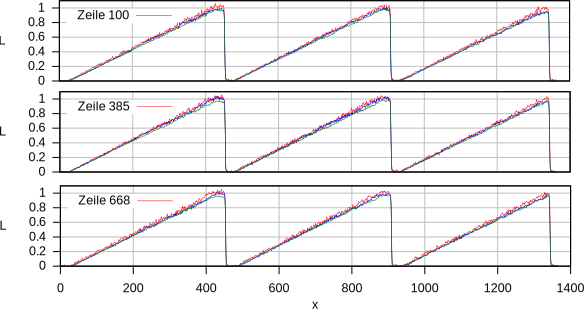
\includegraphics[width=0.7\textwidth]{../graphics/beleuchtung/verify_lenovo_ramps_plot.svg}
    
    \caption[Evaluation der LDR-Beleuchtung (Ursprung): Heatmap]{
     Die Strahldichteverteilung $L_c$ im Ursprung der Szene, beim Erzeugen von einer LDR-Beleuchtung. Als Vorgabe $L_r$ wurden drei linearen Rampen verwendet, die jeweils mit einem Abstand voneinander getrennt sind.
        Die Linienplots zeigen die Strahldichte von drei Bildschirmzeilen.
      Die Messwerte zeigen, dass sowohl die radiometrische Kalibrierung als auch die Berechnung der LDR-Beleuchtung funktioniert: 
     $L_c$ entspricht weitgehend der linearen Eingabe.
     Es gibt jedoch eine geringe Abweichungen zwischen den Farbkanälen, die mit dem Kanalübersprechen (siehe Abschnitt \ref{radiometrisches_modell}) erklärt werden kann.
     Das Rauschen in den Messdaten wird weitgehend durch den Kamera-Sensor verursacht. Es kann jedoch nicht ausgeschlossen werden, dass auch der Bildschirm daran beteiligt ist.

    } 
     \label{fig:ramps_map}
   \end{figure}
   
    Die so erzeugte Strahldichte wurde dann mit der DSLR-Kamera im Ursprung gemessen und ist in Abbildung \ref{fig:ramps_map} dargestellt.
   Damit winkelabhängige Effekte ausgeschlossen werden können, wurde die Aufnahme direkt im Anschluss zur radiometrischen Kalibrierung durchgeführt und die Kamera dazwischen nicht bewegt.
    

 %%%%%%% angular 
    In der Praxis kann der handgehaltene Bildschirm nicht mit dem exakten Winkel ausgerichtet werden, weshalb die Annahmen die bei der Kalibrierung getroffen wurde, verletzt werden.
    Da der Blickwinkel einen Einfluss auf das Ansprechverhalten hat, wurde die LDR-Beleuchtung nicht nur im Ursprung, sondern auch unter verschiedenen Winkeln gemessen.
    Die Kamera wurde dabei jeweils 5$^\circ$ in die horizontale, und in die vertikale Richtung geneigt (siehe Abbildung \ref{fig:angles}). 

 
   \begin{figure}[h]
    \centering
    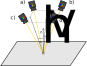
\includegraphics[width=0.45\textwidth]{../graphics/beleuchtung/angle_evaluation_angles.svg}
    \caption[Evaluation der LDR Beleuchtung (Winkel): Aufnahmewinkel]{Zur Evaluation der Blickwinkelabhänigkeit bei einer LDR-Beleuchtung wurde die Strahldichte $L_c$ aus vier unterschiedlichen Positionen aufgenommen. Die Kamera wurde dazu bei der Aufnahme horizontal um $\alpha_h=\pm5^\circ$ und vertikal um $\alpha_v=\pm5^\circ$ geneigt. }
    \label{fig:angles}
   \end{figure}
       
    Die vier Diagramme in Abbildung \ref{fig:ramps_angular} zeigen $L_c$, gemessen aus den vier Positionen a) - d). 
    Der Abstand betrug dabei $r_l=$50 cm.
   Man sieht dass der Blickwinkel einen sehr großen Einfluss auf das Ansprechverhalten hat, da der Laptopbildschirm auf der TN-Technologie basiert.
    Nimmt man an, dass er bei der Beleuchtung immer so ausgerichtet ist, dass $|\alpha_h| < 5^\circ$ und $|\alpha_v| < 5^\circ$ gilt, dann ist mit einer Abweichung von $\pm$20\% zu rechnen.
    
    

   \begin{figure}[h]
    \centering
    \begin{tabular}{cc}
     \includegraphics[width=0.49\textwidth]{../graphics/beleuchtung/verify_angular_h+5,v+5_ramps_map.png}
    &
     \includegraphics[width=0.49\textwidth]{../graphics/beleuchtung/verify_angular_h-5,v+5_ramps_map.png}
    \\ 
     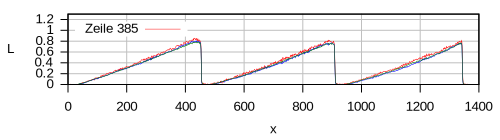
\includegraphics[width=0.49\textwidth]{../graphics/beleuchtung/verify_angular_h+5,v+5_ramps_plot_384.svg}
    & 
     \includegraphics[width=0.49\textwidth]{../graphics/beleuchtung/verify_angular_h-5,v+5_ramps_plot_384.svg}
    \\
   
    a) $\alpha_h=+5^\circ$,  $\alpha_v=+5^\circ$ & 
    b) $\alpha_h=-5^\circ$,  $\alpha_v=+5^\circ$ \\ 
    & \\
     \includegraphics[width=0.49\textwidth]{../graphics/beleuchtung/verify_angular_h+5,v-5_ramps_map.png}
     &
     \includegraphics[width=0.49\textwidth]{../graphics/beleuchtung/verify_angular_h-5,v-5_ramps_map.png}
     \\
     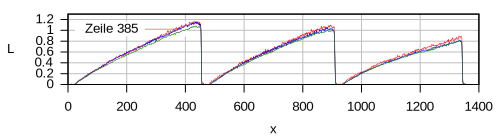
\includegraphics[width=0.49\textwidth]{../graphics/beleuchtung/verify_angular_h+5,v-5_ramps_plot_384.svg}
      &
     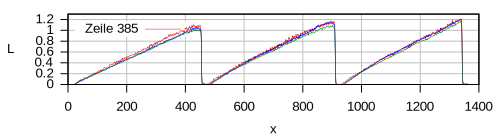
\includegraphics[width=0.49\textwidth]{../graphics/beleuchtung/verify_angular_h-5,v-5_ramps_plot_384.svg}
    \\
    c) $\alpha_h=+5^\circ$,  $\alpha_v=-5^\circ$ & 
    d) $\alpha_h=-5^\circ$,  $\alpha_v=-5^\circ$ \\ 
    & \\
    \end{tabular}
    \caption[Evaluation der LDR-Beleuchtung (Winkel): Diagramme]{
      Die LDR-Beleuchtung, gemessen aus den vier Blickwinkeln a)-d) (siehe Abbildung \ref{fig:angles}). Die Graphen zeigen jeweils die Strahldichte der mittleren Pixelzeile. 
      Dass Ansprechverhalten ist stark winkelabhängig: Man kann deutlich erkennen, dass die vertikale Ausrichtung den \emph{Verlauf} der Kurven beeinflusst.
      Die horizontale Ausrichtung wirkt sich dagegen auf die \emph{maximale Strahldichte} aus.
      }
     \label{fig:ramps_angular}
   \end{figure}
   


     
%%%%%%%%%%%%%%%%%%%%%%%%%%%%%%%%%%%%%%%%%%%%%%%%%%%%%%%%%%%%%%%

    \subsection{Evaluation: HDR-Beleuchtung} 
      In diesem Abschnitt soll gezeigt werden, dass die HDR-Sequenz auch in der Praxis funktioniert und mit ihr der Dynamikbereich des Bildschirms vergrößert werden kann.
      Hierzu wurde eine HDR-Beleuchtung mit verschiedenen Sequenzenlängen erzeugt und gemessen. 
      Als Eingabe für den HDR-Algorithmus kam eine Exponentialrampe zum Einsatz, die Werte zwischen $10^{-3}$ und $1$ beinhaltet, also einen Dynamikbereich von 1000:1 besitzt.
      Die erzeugte HDR-Beleuchtung wurde über die Reflexion an einer schwarzen Billardkugel gemessen, damit längere Belichtungszeiten und somit längere HDR-Sequenzen möglich sind. 
      Die Kugel hatte dabei einen Durchmesser von 6 cm und wurde so platziert dass der Ursprung im Zentrum der Reflexion liegt. 
   
   \pagebreak
      Abbildung \ref{fig:hdr_eval} zeigt die mit einer DSLR-Kamera gemessene Strahldichte für die Sequenzlängen 1, 10, 20, und 100.
      Da die Kamera einen eingeschränkten Dynamikbereich besitzt, wurde die längste Sequenz auch mit einer HDR-Aufnahme (10/20/30 Sekunden) aufgenommen,
      längere Belichtungszeiten waren in dieser Konfiguration nicht möglich.
     
      
   \begin{figure}[H]
    \centering
    \begin{tabular}{cc}
     \includegraphics[width=0.34\textwidth]{../graphics/hdr_beleuchtung/hdr_luminance_logmap_single.png} &
     \includegraphics[width=0.34\textwidth]{../graphics/hdr_beleuchtung/hdr_luminance_logmap_size10.png} \\
     a) 1 Frame& b) 10 Frames \\ 
    & \\
     \includegraphics[width=0.34\textwidth]{../graphics/hdr_beleuchtung/hdr_luminance_logmap_size20.png} &
     \includegraphics[width=0.34\textwidth]{../graphics/hdr_beleuchtung/hdr_luminance_logmap_size100.png} \\
     c) 20 Frames & d) 100 Frames \\
    & \\
   \multicolumn{2}{c}{     \includegraphics[width=0.34\textwidth]{../graphics/hdr_beleuchtung/hdr_luminance_logmap_size100hdr.png}  }\\
   \multicolumn{2}{c}{      e) 100 Frames (HDR-Aufnahme)}\\
    & \\
   \end{tabular} 
    \caption[Evaluation der HDR-Sequenz]{
        Zur Evaluation wurden HDR-Beleuchtungen mit verschieden langen Sequenzen erzeugt und über die Reflexion an einer schwarzen Billardkugel aufgenommen.
        Als Eingabe $L_r$ wurde eine Exponentialrampe verwendet, die Werten zwischen $10^{-3}$ und $1$ beinhaltet ($R=1000:1$). 
        Die Heatmaps zeigen die Strahldichte auf einer logarithmischen Skala, weshalb die Rampe im Plot (im Optimalfall) einen linearen Verlauf besitzen muss.
      Man sieht, dass sich mit längeren Sequenzen kleinere Strahldichtewerte erzeugen lassen - der Dynamikbereich kann folglich vergrößert werden.
      Für eine echte HDR-Beleuchtung werden jedoch sehr viele Frames benötigt:
      Selbst mit $m=100$ liegt der Dynamikbereich des Laptopbildschirms noch deutlich unter 1000:1.

 } 
    \label{fig:hdr_eval}
   \end{figure}
   
      
      Da die Framerate begrenzt ist, mit der die Sequenz angezeigt werden kann, wären für eine wirkliche HDR-Beleuchtung sehr lange Belichtungszeiten notwendig.
      Mit einem handgehaltenen Bildschirm ist dies in der Praxis, wenn der Beleuchtungsablauf aus Kapitel \ref{complete} verwendet wird, nicht umsetzbar, da der Benutzer häufig zu weit von der Position abdriften würde.

      

%%%%%%%%%%%%%%%%%%%%%%%%%%%%%%%%%%%%%%%%%%%%%%%%%%%%%%%%%%%%%%%
      
   \subsection{Evaluation: Überlappungen}
      
      Damit bei der vollständigen Beleuchtung eine zusammenhängende Lichtfläche ohne Lücken oder helle Flecken erzeugt werden kann, muss nicht nur die tatsächliche Bildschirmposition sehr genau bekannt sein, der Benutzer muss ihn theoretisch auch absolut still halten.
      Die Breite der linearen Rampen, mit den die Teilbeleuchtungen ineinander übergeblendet werden, hängt zum Einen von der Genauigkeit der Positionsbestimmung, und zum Anderen von dem Bewegungsspielraum ab, den man bei der Beleuchtung zulässt.
      Die Genauigkeit der Positionsbestimmung kann nur mit hohem Aufwand vollständig evaluiert werden, weshalb die Überlappungsberechnung nur anhand zweier Bildschirmpositionen untersucht wurde.
      Für eine vollständige Evaluation müsste nicht nur jede mögliche Bildschirmposition, sondern auch jeder Ausrichtungswinkel untersucht werden.
 
      Zur Evaluation wurde eine Rampenbreite von 80 Pixel gewählt, was im Falle des Laptops 1,7 cm entspricht, und zwei überlappende Teilbeleuchtungen einmal mit Rampe, und einmal ohne erzeugt, und auf einem Chrom-Objekt fotografiert.
      Dabei wurde eine synthetische Environment-Map verwendet, sodass Lücken und Überlappungen deutlich sichtbar gemacht werden können.
        


   \begin{figure}[h]
    \centering
    \begin{tabular}{cc} 
     \includegraphics[height=0.25\textwidth]{../graphics/beleuchtung/overlap_eval_0_map.png} &
     \includegraphics[height=0.25\textwidth]{../graphics/beleuchtung/overlap_eval_0_cube_map.png} \\
      \multicolumn{2}{c}{  a) ohne Rampen } \\
    & \\
%     $s_r=0$ & $s_r=0$ \\
%     \includegraphics[height=0.25\textwidth]{../graphics/beleuchtung/overlap_eval_40_map.png} &
%     \includegraphics[height=0.25\textwidth]{../graphics/beleuchtung/overlap_eval_40_cube_map.png} \\
%     $s_r=40$ & $s_r=40$ \\
     \includegraphics[height=0.25\textwidth]{../graphics/beleuchtung/overlap_eval_80_map.png} &
     \includegraphics[height=0.25\textwidth]{../graphics/beleuchtung/overlap_eval_80_cube_map.png} \\
      \multicolumn{2}{c}{  a) mit Rampen (80 Pixel, 1.7cm) } \\
   \end{tabular}
    \caption[Evaluation der Überlappung von Teilbeleuchtungen]{
          Zwei überlappende Teilbeleuchtungen wurden anhand eine synthetischen Environment-Map erzeugt und über ein Chrom-Objekt, das sich im Ursprung befindet, fotografiert. 
          Die linke Spalte zeigt die Aufnahmen, und die rechte den erzeugten Ausschnitt der Environment-Map.
          In \textbf{a)} wurden die Teilbeleuchtungen nicht ineinander überblendet, in \textbf{b)} wurde eine 80 Pixel breite Rampe verwendet, was in etwa 1.7cm auf dem Bildschirm entspricht.
          Der Bildschirm wurde dabei wie in Abbildung \ref{fig:ablauf_position} dargestellt von Hand gehalten. }
    \label{fig:overlap_maps}
   \end{figure}
         


      Der Bildschirm wurde dabei wie im Beleuchtungsablauf (siehe Abbildung \ref{fig:ablauf_position}) von Hand gehalten.
      In Abbildung \ref{fig:overlap_maps} sind auf der linken Seite die Aufnahme, und auf der rechten Seite der Ausschnitt der Environment-Map dargestellt.
      Man kann sehen, dass ohne ein Überblenden zwischen den Teilbeleuchtungen deutlich sichtbare Artefakte entstehen können. 
      Die Aufnahmen sind leider nicht direkt miteinander vergleichbar, da die Bildschirmposition nicht identisch sind.
      Es kann also keine Aussage über die optimale Breite $s_r$ der Rampen getroffen werden. 
 
       
